%location/filename: tex/fig/ap1.tex
%author: Anders Østevik
%Last edited: 20.05.2016
%#######--Appendix - HSMC-to-VLDB gerber files--#######
%

\documentclass[main.tex]{subfiles}

\begin{document}

\chapter{Basics}

This chapter contains information about basic concepts and devices used in this thesis.

\section{Field Programmable Gate Array} \label{sec:fpga}

A \gls{fpga} is a high density \gls{ic} that is designed to be completely programmable by the customer after manufacturing (i.e. when the chip is shipped and "in the field"). The chips are shipped completely "blank", meaning that there are no pre-programmed logic\footnote{With the exception of \gls{fpga} evaluation boards, which comes shipped with a pre-programmed hardware setup for demo purposes.}. An \gls{fpga} can either be re-programmed using SRAM technology\footnote{Short for Static Random Access Memory, SRAM is a type of volatile memory that uses internal feedback to keep on its data.\cite{weste11} Volatile meaning that the memory loses all the data once the power is switched off.}, or one-time programmed by burning antifuses. The latter method makes it less prone to soft errors when exposed to radiation.\\

\Glspl{fpga} are composed of arrays of \glspl{clb} surrounded by programmable routing resources and I/O pads. A \gls{clb} consists of a \gls{lut} together with a clock and simple write logic, and uses the address bus of the \gls{lut} as the function input pins and the value at the selected address as the function output. \glspl{lut} are considered fast logic, since computing a complex function only requires a single memory lookup. The \gls{lut} can be made out of an SRAM memory-block \cite{weste11}. \\

The \gls{fpga} (section \ref{sec:cyclone}) used in this thesis is a re-programmable type. It stores the user hardware setup in an SRAM memory to configure routing and logic functions (for a permanent program storage, the \gls{fpga} can be configures to store the hardware setup in the on-board flash memory\footnote{A nonvolatile memory type known by its name because of its ability to erase memory blocks all at once "in a flash".\cite{weste11} Nonvolatile meaning that the memory will keep all its data even if the power is switched off.}, which then programs the SRAM when powered on).

\subsection{Hardware Description Language}

The most common way to program an \gls{fpga} is by \gls{hdl}, with the major ones being SystemVerilog and \acrshort{vhdl}. \Gls{hdl} consists of text-based expressions used to describe digital hardware and use this to further simulate and synthesize the hardware described. A hardware module is simulated by applying information at the inputs and then do a check on the corresponding outputs and verify that they behave as intended. Synthesis of hardware means transforming the \gls{hdl} code into a netlist of logic and wire connections describing the hardware. This can then be compiled into an \gls{fpga} which re-wires the available internal \glspl{clb} according to the given instructions. \glspl{hdl} have become more and more useful as system complexity have increased \cite{weste11}. The hardware described in this thesis is done using \acrshort{vhdl}, a strongly typed \gls{hdl} that is known for its capability of describing parallel processes.

Below is a small example describing the logic of a D Flip-Flop using \acrshort{vhdl}:

\lstset { %
    language=VHDL,
    backgroundcolor=\color{black!5}, % set backgroundcolor
    basicstyle=\footnotesize,% basic font setting
}

\begin{lstlisting}[frame=single] 
-- Example of a D Flip-Flop triggered on the rising edge of the clock.
library IEEE; 
use IEEE.std_logic_1164.all; 
 
entity DFF_high is 
  port( 
    D : in STD_LOGIC; 
    Q : out STD_LOGIC; 
    Qbar : out STD_LOGIC; 
    RESET : in STD_LOGIC; 
    CLK : in STD_LOGIC 
  ); 
end DFF_high; 
 
architecture rtl of DFF_high is 
begin 
 
process(CLK,RESET) 
begin 
  if (RESET='1') then 
    Q <= '0'; 
    Qbar <= '1'; 
  elsif (CLK'event and CLK='1') then -- Can also use rising_edge(clk)
    Q <= D; 
    Qbar <= not D; 
  end if; 
end process;
  
end rtl; 
\end{lstlisting}


\section{RS-232} \label{ap:rs232}

RS-232 standard is a transmission protocol for full duplex, serial transmitting and receiving of data. The standard defines electrical characteristics and timing of signals, the "meaning" of the signal, and also physical size and pin-out for connectors.
For communications to work properly, the \gls{dte}, in this case the \acrshort{pc}; and the\gls{dce}, in this case the \gls{fpga}, needs to agree on the same data-packet settings, i.e the baud rate, the number of data bits, any additional parity bit and the number of stop bits.\\

A typical RS-232 data-packet consists of a start bit, followed by 5, 7 or 8 data bits; 1 parity bit, for error checking; and 1 or 2 stop bits, indicating that the transmission is done. The start bit is typically a logical low and the stop bit(s) high (this is usually the case, but can be system dependent). The transmission line remains high until the start bit pulls it down low, and the data transfer begins until the stop bit is reached. The line is then kept high until a new start bit pulls it low again for a new byte to be transfered. Data-packets are often described in the form: $19200-8-N-1$, which simply means $19200~ \bit\per\second$, $8~ data~ bits$, $No~ parity$ and $1~ stop~ bit$. Figure \ref{fig:rs232} demonstrates a typical RS-232 signal.\\

\begin{figure}[!h]
\begin{center}
\begin{tikzpicture}

\timing [
yscale=2.0,
timing/wscale=3.0,
timing/inline 
node/.style={below left, font=\sffamily\scriptsize}
] at (0,0)
{
H N {$Idle$}
L N {$Start$} 
D {$D_0$} 
D {$D_1$} 
D {$D_2$} 
D {$D_3$} 
D {$D_4$} 
D {$D_5$} 
D {$D_6$}  
D {$D_7$} 
D {$Parity$} 
H N{$Stop$}
%L H N[xscale=.8]{ACK} 
H N{$Idle$}
};

\end{tikzpicture}

\caption{Example of an RS-232 signal with 8 data bits, 1 parity bit (Odd, Even or No parity) and 1 stop bit.}
\label{fig:rs232}

\end{center}
\end{figure}


\end{document}
